\documentclass[a4paper, 12pt]{article}

\usepackage[utf8]{inputenc}
\usepackage[T5]{fontenc}
\usepackage[vietnamese]{babel}

\usepackage[a4paper,margin=24mm]{geometry}
\usepackage[skip=10pt plus1pt, indent=20pt]{parskip}
\usepackage{indentfirst}
\usepackage{fancyhdr}
\usepackage{titlesec}
\usepackage{tocbasic}

\usepackage{amsmath,amssymb}
\usepackage{textcomp}
\usepackage{gensymb}

\usepackage{graphicx}
\usepackage{subfig}
\usepackage{subcaption}
\usepackage{xcolor}

\usepackage[colorlinks=true,allcolors=blue,urlcolor=magenta]{hyperref}

\usepackage{minted}
\usepackage{listings}
\usepackage{verbatim}

\usepackage{relsize}
\usepackage{array}

\usepackage[colorinlistoftodos]{todonotes}

\usepackage{lipsum}
\usepackage[normalem]{ulem}
\usepackage{xparse}

\NewDocumentCommand{\myrule}{O{1pt} O{2pt} O{black}}{%
  \par\nobreak%
  \kern\the\prevdepth%
  \kern#2
  {\color{#3}\hrule height #1 width\hsize} 
  \kern#2
  \nointerlineskip%
}

\usepackage[section]{placeins}

\usepackage{booktabs}    
\usepackage{colortbl}   
\newcommand{\myrowcolour}{\rowcolor[gray]{0.925}} 

\DeclareTOCStyleEntry[
  indent=12pt,
  level=1
]{largetocline}{section}

\setlength{\marginparwidth}{2cm}

\begin{document}
\thispagestyle{empty}
\begin{titlepage}
  \begin{center}
    \textbf{\LARGE ĐẠI HỌC QUỐC GIA}\\
    \textbf{\LARGE THÀNH PHỐ HỒ CHÍ MINH}\\[0.5cm]
    \vspace{20pt}
    \textbf{\large TRƯỜNG ĐẠI HỌC KHOA HỌC TỰ NHIÊN}\\[0.2cm]
    \textbf{\large KHOA CÔNG NGHỆ THÔNG TIN}\\[0.2cm]
    \vspace{20pt}
    
\includegraphics[width=0.4\textwidth,keepaspectratio]{imgs/logo.png}

    \par
    \vspace{20pt}
    \textbf{\Large MTH00057 - Toán ứng dụng và thống kê cho Công nghệ thông tin}\\
    \vspace{15pt}
    \myrule[1pt][7pt]
    \textbf{\LARGE BÁO CÁO ĐỒ ÁN 3}\\
    \vspace{15pt}
    \textbf{\Large Linear Regression}\\
    \vspace{10pt}
    \myrule[1pt][7pt]
    \vspace{25pt}

    \begin{tabular}{c@{\hspace{2cm}}c}
      \textbf{Họ tên} & \textbf{MSSV} \\
      Bùi Minh Duy    & 23127040      \\
    \end{tabular}

    \vspace{10pt}
    \textbf {Giảng viên hướng dẫn}\\[0.2cm]
    Nguyễn Văn Quang Huy \\ Trần Hà Sơn \\ Nguyễn Đình Thúc\\ Nguyễn Ngọc Toàn

    \vspace{25pt}
    \today

  \end{center}
\end{titlepage}

\newpage

\tableofcontents\thispagestyle{empty}
\newpage

\section{Ý tưởng thực hiện}

\subsection{Tổng quan về đồ án}
Đồ án 3 tập trung vào việc xây dựng mô hình \textbf{Linear Regression} để dự đoán chỉ số thành tích học tập của sinh viên (Academic Student Performance Index). Mục tiêu chính là tìm hiểu các yếu tố ảnh hưởng đến kết quả học tập và xây dựng các mô hình dự đoán hiệu quả.

\subsection{Input và Output}
\textbf{Input:}
\begin{itemize}
	\item \textbf{Tập huấn luyện:} p03.train.csv (9000 mẫu)
	\item \textbf{Tập kiểm tra:} p03.test.csv (1000 mẫu)
	\item \textbf{Đặc trưng đầu vào:} 5 thuộc tính
	      \begin{itemize}
		      \item Hours Studied: Số giờ học tập
		      \item Previous Scores: Điểm số các bài kiểm tra trước
		      \item Extracurricular Activities: Hoạt động ngoại khóa (0/1)
		      \item Sleep Hours: Số giờ ngủ
		      \item Sample Question Papers Practiced: Số bài kiểm tra mẫu đã luyện tập
	      \end{itemize}
\end{itemize}

\textbf{Output:}
\begin{itemize}
	\item \textbf{Dự đoán Performance Index:} Chỉ số thành tích học tập được dự đoán cho từng sinh viên
	\item \textbf{Các mô hình hồi quy tuyến tính} với độ chính xác khác nhau
	\item \textbf{Đánh giá hiệu suất} bằng độ đo MSE (Mean Squared Error)
	\item \textbf{Công thức toán học} cho mỗi mô hình với các hệ số được tính toán
\end{itemize}

\subsection{Mục tiêu}
\begin{enumerate}
	\item \textbf{Phân tích khám phá dữ liệu (EDA):} Hiểu rõ đặc điểm và mối quan hệ giữa các thuộc tính với thành tích học tập
	\item \textbf{Xây dựng mô hình hồi quy tuyến tính:}
	      \begin{itemize}
		      \item Mô hình sử dụng toàn bộ 5 đặc trưng
		      \item Mô hình sử dụng 1 đặc trưng tốt nhất
		      \item Mô hình tùy chỉnh sinh viên tự xây dựng
	      \end{itemize}
	\item \textbf{So sánh và đánh giá:} Tìm ra mô hình có hiệu suất tốt nhất
\end{enumerate}

\subsection{Ý tưởng giải quyết}

\subsubsection{Phương pháp tiếp cận}
\textbf{1. Phân tích khám phá dữ liệu:}
\begin{itemize}
	\item Sử dụng thống kê mô tả để hiểu phân phối dữ liệu
	\item Trực quan hóa bằng các biểu đồ: histogram, boxplot, scatter plot, correlation matrix
	\item Phát hiện outliers và missing values
	\item Phân tích mối tương quan giữa các đặc trưng
\end{itemize}

\textbf{2. Xây dựng mô hình Linear Regression:}
\begin{itemize}
	\item Cài đặt mô hình Linear Regression sử dụng Normal Equation: \(\beta = {(X^{T}X)}^{-1}X^{T}y\)
	\item Áp dụng k-fold Cross Validation để đánh giá độ tin cậy
	\item Sử dụng MSE làm độ đo đánh giá hiệu suất
\end{itemize}

\textbf{3. Kỹ thuật đặc trưng:}
\begin{itemize}
	\item Tạo các đặc trưng mới từ sự kết hợp của các đặc trưng gốc
	\item Áp dụng đặc trưng đa thức
	\item Chuẩn hóa dữ liệu (chuẩn hóa Z-score)
	\item Tạo đặc trưng tương tác để nắm bắt mối quan hệ phức tạp
\end{itemize}

\subsubsection{Kiến trúc hệ thống}
\begin{enumerate}
	\item \textbf{Module xử lý dữ liệu:}
	      \begin{itemize}
		      \item Hàm đọc dữ liệu: Đọc và xử lý dữ liệu từ tập tin CSV
		      \item Hàm trực quan hóa EDA: Tạo 6 biểu đồ phân tích khám phá dữ liệu
		      \item Quản lý biểu đồ: Tự động tạo thư mục và lưu biểu đồ
	      \end{itemize}

	\item \textbf{Module cài đặt mô hình chính:}
	      \begin{itemize}
		      \item Lớp \texttt{LinearRegression}: Cài đặt mô hình hồi quy tuyến tính
		      \item Hàm \texttt{calculate\_mse()}: Tính toán MSE với mảng numpy
		      \item Hàm \texttt{k\_fold\_cross\_validation()}: Đánh giá chéo k-fold với hạt giống ngẫu nhiên
		      \item Hàm \texttt{display\_model\_formula()}: Hiển thị công thức toán học của mô hình
	      \end{itemize}

	\item \textbf{Module kỹ thuật đặc trưng:}
	      \begin{itemize}
		      \item \textbf{Mô hình 1}: Sử dụng 2 đặc trưng tốt nhất
		      \item \textbf{Mô hình 2}: Sử dụng 3 đặc trưng tốt nhất
		      \item \textbf{Mô hình 3}: Đặc trưng bậc 2
		      \item \textbf{Mô hình 4}: Đặc trưng chuẩn hóa Z-score
		      \item \textbf{Mô hình 5}: Đặc trưng tương tác và kỹ thuật
	      \end{itemize}

	\item \textbf{Module đánh giá và báo cáo:}
	      \begin{itemize}
		      \item So sánh cross-validation
		      \item Tính toán MSE trên tập kiểm tra
		      \item Lựa chọn mô hình tốt nhất dựa trên điểm số cross-validation
		      \item Hiển thị công thức với ký hiệu toán học
		      \item Phân tích hiệu suất và nhận xét kết quả
	      \end{itemize}
\end{enumerate}

\subsubsection{Chiến lược lựa chọn đặc trưng}
Dựa trên phân tích EDA, đề xuất các chiến lược:
\begin{itemize}
	\item \textbf{Đặc trưng hàng đầu:} Kết hợp 2-3 đặc trưng có tương quan cao nhất
	\item \textbf{Phương pháp đa thức:} Sử dụng Previous Scores và bình phương của nó
	\item \textbf{Chuẩn hóa:} Chuẩn hóa để cân bằng tầm quan trọng các đặc trưng
	\item \textbf{Đặc trưng tương tác:} Tạo đặc trưng mới phản ánh mối quan hệ phức tạp
	\item \textbf{Đặc trưng kỹ thuật:} Tạo chỉ số tổng hợp như ``hiệu quả học tập'', ``chỉ số cân bằng''
\end{itemize}

\newpage
\section{Chi tiết thực hiện}

\subsection{Cấu trúc chương trình}

\subsubsection{Thư viện sử dụng}
Chương trình sử dụng các thư viện Python sau:
\begin{itemize}
	\item \textbf{pandas}: Xử lý và thao tác dữ liệu dạng DataFrame, đọc tập tin CSV
	\item \textbf{numpy}: Tính toán số học, đại số tuyến tính và các phép toán ma trận
	\item \textbf{matplotlib.pyplot}: Tạo biểu đồ và trực quan hóa dữ liệu
	\item \textbf{seaborn}: Tạo biểu đồ thống kê chuyên sâu và ma trận tương quan
	\item \textbf{os}: Quản lý thư mục, đường dẫn tập tin và hệ thống
\end{itemize}

\subsection{Module xử lý dữ liệu}

\subsubsection{Đọc và xử lý dữ liệu}
\begin{itemize}
	\item Sử dụng \texttt{pd.read\_csv()} để đọc tập tin `p03.train.csv' (9000 mẫu) và `p03.test.csv' (1000 mẫu)
	\item Lưu trữ dữ liệu gốc trong \texttt{train\_raw} và \texttt{test\_raw}
	\item Sử dụng \texttt{drop\_duplicates(keep=`first')} để loại bỏ dữ liệu trùng lặp
	\item Báo cáo chi tiết số lượng dòng ban đầu, số dòng trùng lặp và số dòng còn lại
	\item Lưu dữ liệu đã được làm sạch vào \texttt{train} và \texttt{test}
\end{itemize}

\subsubsection{Phân tích khám phá dữ liệu (EDA)}
Thực hiện phân tích toàn diện trên tập huấn luyện:

\textbf{Thống kê mô tả}:
\begin{itemize}
	\item Sử dụng \texttt{train.info()} để kiểm tra kiểu dữ liệu và missing values
	\item Sử dụng \texttt{train.describe()} để có thống kê tổng quan
	\item Kiểm tra \texttt{train.isnull().sum()} để xác nhận không có giá trị thiếu
\end{itemize}

\textbf{Trực quan hóa dữ liệu} - Tạo 6 biểu đồ chính:
\begin{itemize}
	\item \textbf{Figure 1}: Distribution of Performance Index - Biểu đồ phân phối của biến mục tiêu
	\item \textbf{Figure 2}: Boxplots for numerical features - Biểu đồ hộp cho các đặc trưng số
	\item \textbf{Figure 3}: Distribution of Extracurricular Activities - Phân phối hoạt động ngoại khóa
	\item \textbf{Figure 4}: Correlation Matrix - Ma trận tương quan giữa các đặc trưng
	\item \textbf{Figure 5}: Scatter plots relationships - Biểu đồ phân tán mối quan hệ với Performance Index
	\item \textbf{Figure 6}: Performance comparison by Extracurricular - So sánh hiệu suất theo hoạt động ngoại khóa
\end{itemize}

\subsection{Module cài đặt mô hình chính}

\subsubsection{Lớp \texttt{LinearRegression}}
\textbf{Mục đích}: Cài đặt hoàn chỉnh mô hình hồi quy tuyến tính sử dụng Normal Equation.

\textbf{Thuộc tính}:
\begin{itemize}
	\item \texttt{coefficients}: Mảng các hệ số \(\beta_1, \beta_2, ..., \beta_n\)
	\item \texttt{intercept}: Hệ số chặn \(\beta_0\)
	\item \texttt{feature\_names}: Danh sách tên các đặc trưng
\end{itemize}

\textbf{Phương thức \texttt{fit(X, y)}}:
\begin{enumerate}
	\item Chuyển đổi dữ liệu đầu vào thành numpy arrays
	\item Lưu trữ tên đặc trưng nếu X là DataFrame
	\item Thêm cột bias (cột toàn số 1) cho intercept: \texttt{X\_with\_bias}
	\item Áp dụng Normal Equation: \(\beta = {(X^{T}X)}^{-1}X^{T}y\)
	      \begin{itemize}
		      \item Tính \texttt{XtX = np.dot(X\_with\_bias.T, X\_with\_bias)}
		      \item Tính \texttt{XtX\_inv = np.linalg.inv(XtX)}
		      \item Tính \texttt{Xty = np.dot(X\_with\_bias.T, y)}
		      \item Kết quả: \texttt{beta = np.dot(XtX\_inv, Xty)}
	      \end{itemize}
	\item Xử lý ngoại lệ ma trận suy biến bằng pseudo-inverse
	\item Tách intercept và coefficients từ vector beta
\end{enumerate}

\textbf{Phương thức \texttt{predict(X)}}:
\begin{itemize}
	\item Áp dụng công thức: \(y = \beta_0 + \beta_1x_1 + \beta_2x_2 + \cdots + \beta_{n}x_{n}\)
	\item Sử dụng \texttt{np.dot(X, self.coefficients)} để tính tích vô hướng
	\item Trả về mảng dự đoán
\end{itemize}

\subsubsection{Hàm \texttt{calculate\_mse()}}
\textbf{Mục đích}: Tính Mean Squared Error để đánh giá hiệu suất mô hình.

\textbf{Công thức toán học}:
\[MSE = \frac{1}{n}\sum_{i=1}^{n}{(y_i - \hat{y_i})}^2\]

\textbf{Thực hiện}:
\begin{itemize}
	\item Chuyển đổi \texttt{y\_true} và \texttt{y\_pred} thành numpy arrays
	\item Tính số lượng mẫu: \texttt{n = len(y\_true)}
	\item Áp dụng công thức: \texttt{mse = np.sum((y\_true - y\_pred) ** 2) / n}
\end{itemize}

\subsubsection{Hàm \texttt{k\_fold\_cross\_validation()}}
\textbf{Mục đích}: Thực hiện đánh giá chéo k-fold để đánh giá độ tin cậy mô hình.

\textbf{Tham số}:
\begin{itemize}
	\item \texttt{X}: Ma trận đặc trưng
	\item \texttt{y}: Vector mục tiêu
	\item \texttt{k=5}: Số fold (mặc định 5) - Cân bằng giữa độ chính xác và chi phí tính toán
	\item \texttt{random\_state=42}: Hạt giống ngẫu nhiên (giá trị phổ biến trong Machine Learning) để đảm bảo tái tạo kết quả
\end{itemize}

\textbf{Quy trình thực hiện}:
\begin{enumerate}
	\item Thiết lập hạt giống ngẫu nhiên: \texttt{np.random.seed(random\_state)}
	\item Tạo và xáo trộn chỉ số mẫu: \texttt{np.random.shuffle(indices)}
	\item Chia dữ liệu thành k folds với \texttt{fold\_size = n\_samples // k}
	\item Với mỗi fold i:
	      \begin{itemize}
		      \item Xác định chỉ số test: từ \texttt{i * fold\_size} đến \texttt{(i+1) * fold\_size}
		      \item Chỉ số train: tất cả mẫu còn lại
		      \item Chia dữ liệu theo chỉ số
		      \item Huấn luyện mô hình LinearRegression trên fold train
		      \item Dự đoán trên fold test và tính MSE
	      \end{itemize}
	\item Trả về MSE trung bình: \texttt{np.mean(mse\_scores)}
\end{enumerate}

\subsubsection{Hàm \texttt{display\_model\_formula()}}
\textbf{Mục đích}: Hiển thị công thức hồi quy dưới dạng toán học dễ đọc.

\textbf{Thực hiện}:
\begin{itemize}
	\item Bắt đầu với intercept: \texttt{f"Student Performance = \{model.intercept:.3f\}"}
	\item Duyệt qua từng đặc trưng và hệ số tương ứng
	\item Xử lý dấu "+/-" tự động dựa trên giá trị hệ số
	\item Định dạng: \texttt{f"\{sign\}\{coef:.3f\}×\{feature\}"}
	\item In ra công thức hoàn chỉnh
\end{itemize}

\subsection{Module kỹ thuật đặc trưng}

\subsubsection{Thiết kế 5 mô hình tùy chỉnh}

\textbf{Mô hình 1: Top 2 đặc trưng}
\begin{itemize}
	\item \textbf{Hàm}: \texttt{create\_model1\_features(X)}
	\item \textbf{Đặc trưng}: Hours Studied + Previous Scores
	\item \textbf{Cơ sở}: Dựa trên phân tích tương quan cao nhất từ EDA
	\item \textbf{Thực hiện}: \texttt{return X[[`Hours Studied', `Previous Scores']]}
\end{itemize}

\textbf{Mô hình 2: Top 3 đặc trưng}
\begin{itemize}
	\item \textbf{Hàm}: \texttt{create\_model2\_features(X)}
	\item \textbf{Đặc trưng}: Hours Studied + Previous Scores + Extracurricular Activities
	\item \textbf{Cơ sở}: Mở rộng từ Model 1 với thêm yếu tố hoạt động ngoại khóa
	\item \textbf{Thực hiện}: \texttt{return X[[`Hours Studied', `Previous Scores', `Extracurricular Activities']]}
\end{itemize}

\textbf{Mô hình 3: Đặc trưng đa thức}
\begin{itemize}
	\item \textbf{Hàm}: \texttt{create\_model3\_features(X)}
	\item \textbf{Đặc trưng}: Previous Scores + Previous Scores²
	\item \textbf{Cơ sở}: Nắm bắt mối quan hệ phi tuyến
	\item \textbf{Thực hiện}:
	      \begin{itemize}
		      \item \texttt{X\_new = X[[`Previous Scores']].copy()}
		      \item \texttt{X\_new[`Previous\_Scores\_squared'] = X[`Previous Scores'] ** 2}
	      \end{itemize}
\end{itemize}

\textbf{Mô hình 4: Chuẩn hóa Z-score}
\begin{itemize}
	\item \textbf{Hàm}: \texttt{create\_model4\_features(X)}
	\item \textbf{Đặc trưng}: Hours Studied và Previous Scores được chuẩn hóa
	\item \textbf{Công thức chuẩn hóa}: \(z = \frac{x - \mu}{\sigma}\)
	\item \textbf{Thực hiện}:
	      \begin{itemize}
		      \item Tính mean và std cho mỗi đặc trưng
		      \item \texttt{Hours\_Normalized = (Hours - mean) / std}
		      \item \texttt{Previous\_Normalized = (Previous - mean) / std}
	      \end{itemize}
\end{itemize}

\textbf{Mô hình 5: Đặc trưng tương tác và kỹ thuật}
\begin{itemize}
	\item \textbf{Đặc trưng kỹ thuật:}
	\begin{itemize}
		\item \textbf{Hours\_x\_Previous}: \texttt{X[`Hours Studied'] * X[`Previous Scores']}
		\item \textbf{Study\_Efficiency}: \texttt{X[`Hours Studied'] * X[`Sample Question Papers Practiced']}
		\item \textbf{Total\_Capability}: \texttt{X[`Previous Scores'] + X[`Extracurricular Activities'] * 10}
		\item \textbf{Balance\_Index}: \texttt{X[`Previous Scores'] / (X[`Hours Studied'] + 1)}
	\end{itemize}
	\item \textbf{Ý nghĩa}:
	\begin{itemize}
		\item Tương tác giữa số giờ học và điểm số trước đó
		\item Hiệu quả học tập qua việc luyện tập
		\item Tổng năng lực với bonus từ hoạt động ngoại khóa (nhân 10 để tạo trọng số có ý nghĩa so với Previous Scores)
		\item Chỉ số cân bằng đánh giá hiệu quả (tránh chia 0 bằng cách cộng thêm 1 vào Hours Studied)
	\end{itemize}
\end{itemize}

\subsection{Module đánh giá và báo cáo}

\subsubsection{Yêu cầu 2a: Mô hình 5 đặc trưng}
\textbf{Quy trình thực hiện}:
\begin{enumerate}
	\item Khởi tạo mô hình: \texttt{model\_2a = LinearRegression()}
	\item Huấn luyện: \texttt{model\_2a.fit(X\_train, y\_train)}
	\item Dự đoán: \texttt{y\_pred\_2a = model\_2a.predict(X\_test)}
	\item Đánh giá: \texttt{mse\_2a = calculate\_mse(y\_test, y\_pred\_2a)}
	\item Hiển thị công thức: \texttt{display\_model\_formula(model\_2a, X\_train.columns)}
\end{enumerate}

\subsubsection{Yêu cầu 2b: Đặc trưng tốt nhất}
\textbf{Quy trình so sánh}:
\begin{enumerate}
	\item Định nghĩa danh sách 5 đặc trưng
	\item Với mỗi đặc trưng:
	      \begin{itemize}
		      \item Tạo \texttt{X\_single = X\_train[[feature]]}
		      \item Thực hiện 5-fold cross validation
		      \item Lưu kết quả MSE vào dictionary
	      \end{itemize}
	\item Tìm đặc trưng tốt nhất: \texttt{min(cv\_results, key=cv\_results.get)}
	\item Huấn luyện lại mô hình với đặc trưng tốt nhất
	\item Đánh giá trên tập test
\end{enumerate}

\subsubsection{Yêu cầu 2c: Mô hình tùy chỉnh}
\textbf{Quy trình đánh giá}:
\begin{enumerate}
	\item Định nghĩa dictionary chứa 5 mô hình và hàm tạo đặc trưng
	\item Với mỗi mô hình:
	      \begin{itemize}
		      \item Gọi hàm tạo đặc trưng: \texttt{X\_features = feature\_func(X\_train)}
		      \item Thực hiện 5-fold cross validation
	      \end{itemize}
	\item Lựa chọn mô hình tốt nhất dựa trên MSE thấp nhất
	\item Huấn luyện lại trên toàn bộ tập train
	\item Đánh giá trên tập test
\end{enumerate}
\newpage
\section{Kết quả và Kết luận}

\subsection{Kết quả Phân tích Khám phá Dữ liệu}

\subsubsection{Thông tin tổng quan về dữ liệu}
Sau quá trình đọc và làm sạch dữ liệu:
\begin{itemize}
	\item \textbf{Tập huấn luyện}: Còn lại 8896 mẫu (đã loại 103 mẫu trùng lặp)
	\item \textbf{Tập kiểm tra}: Còn lại 999 mẫu (đã loại 1 mẫu trùng lặp)
	\item \textbf{Đặc trưng}: 5 đặc trưng đầu vào và 1 biến mục tiêu (Performance Index)
	\item \textbf{Chất lượng dữ liệu}: Không có giá trị thiếu (missing values)
\end{itemize}

\subsubsection{Phân tích trực quan hóa dữ liệu}
Từ 6 biểu đồ được tạo ra trong quá trình EDA:

\begin{figure}[H]
	\centering
	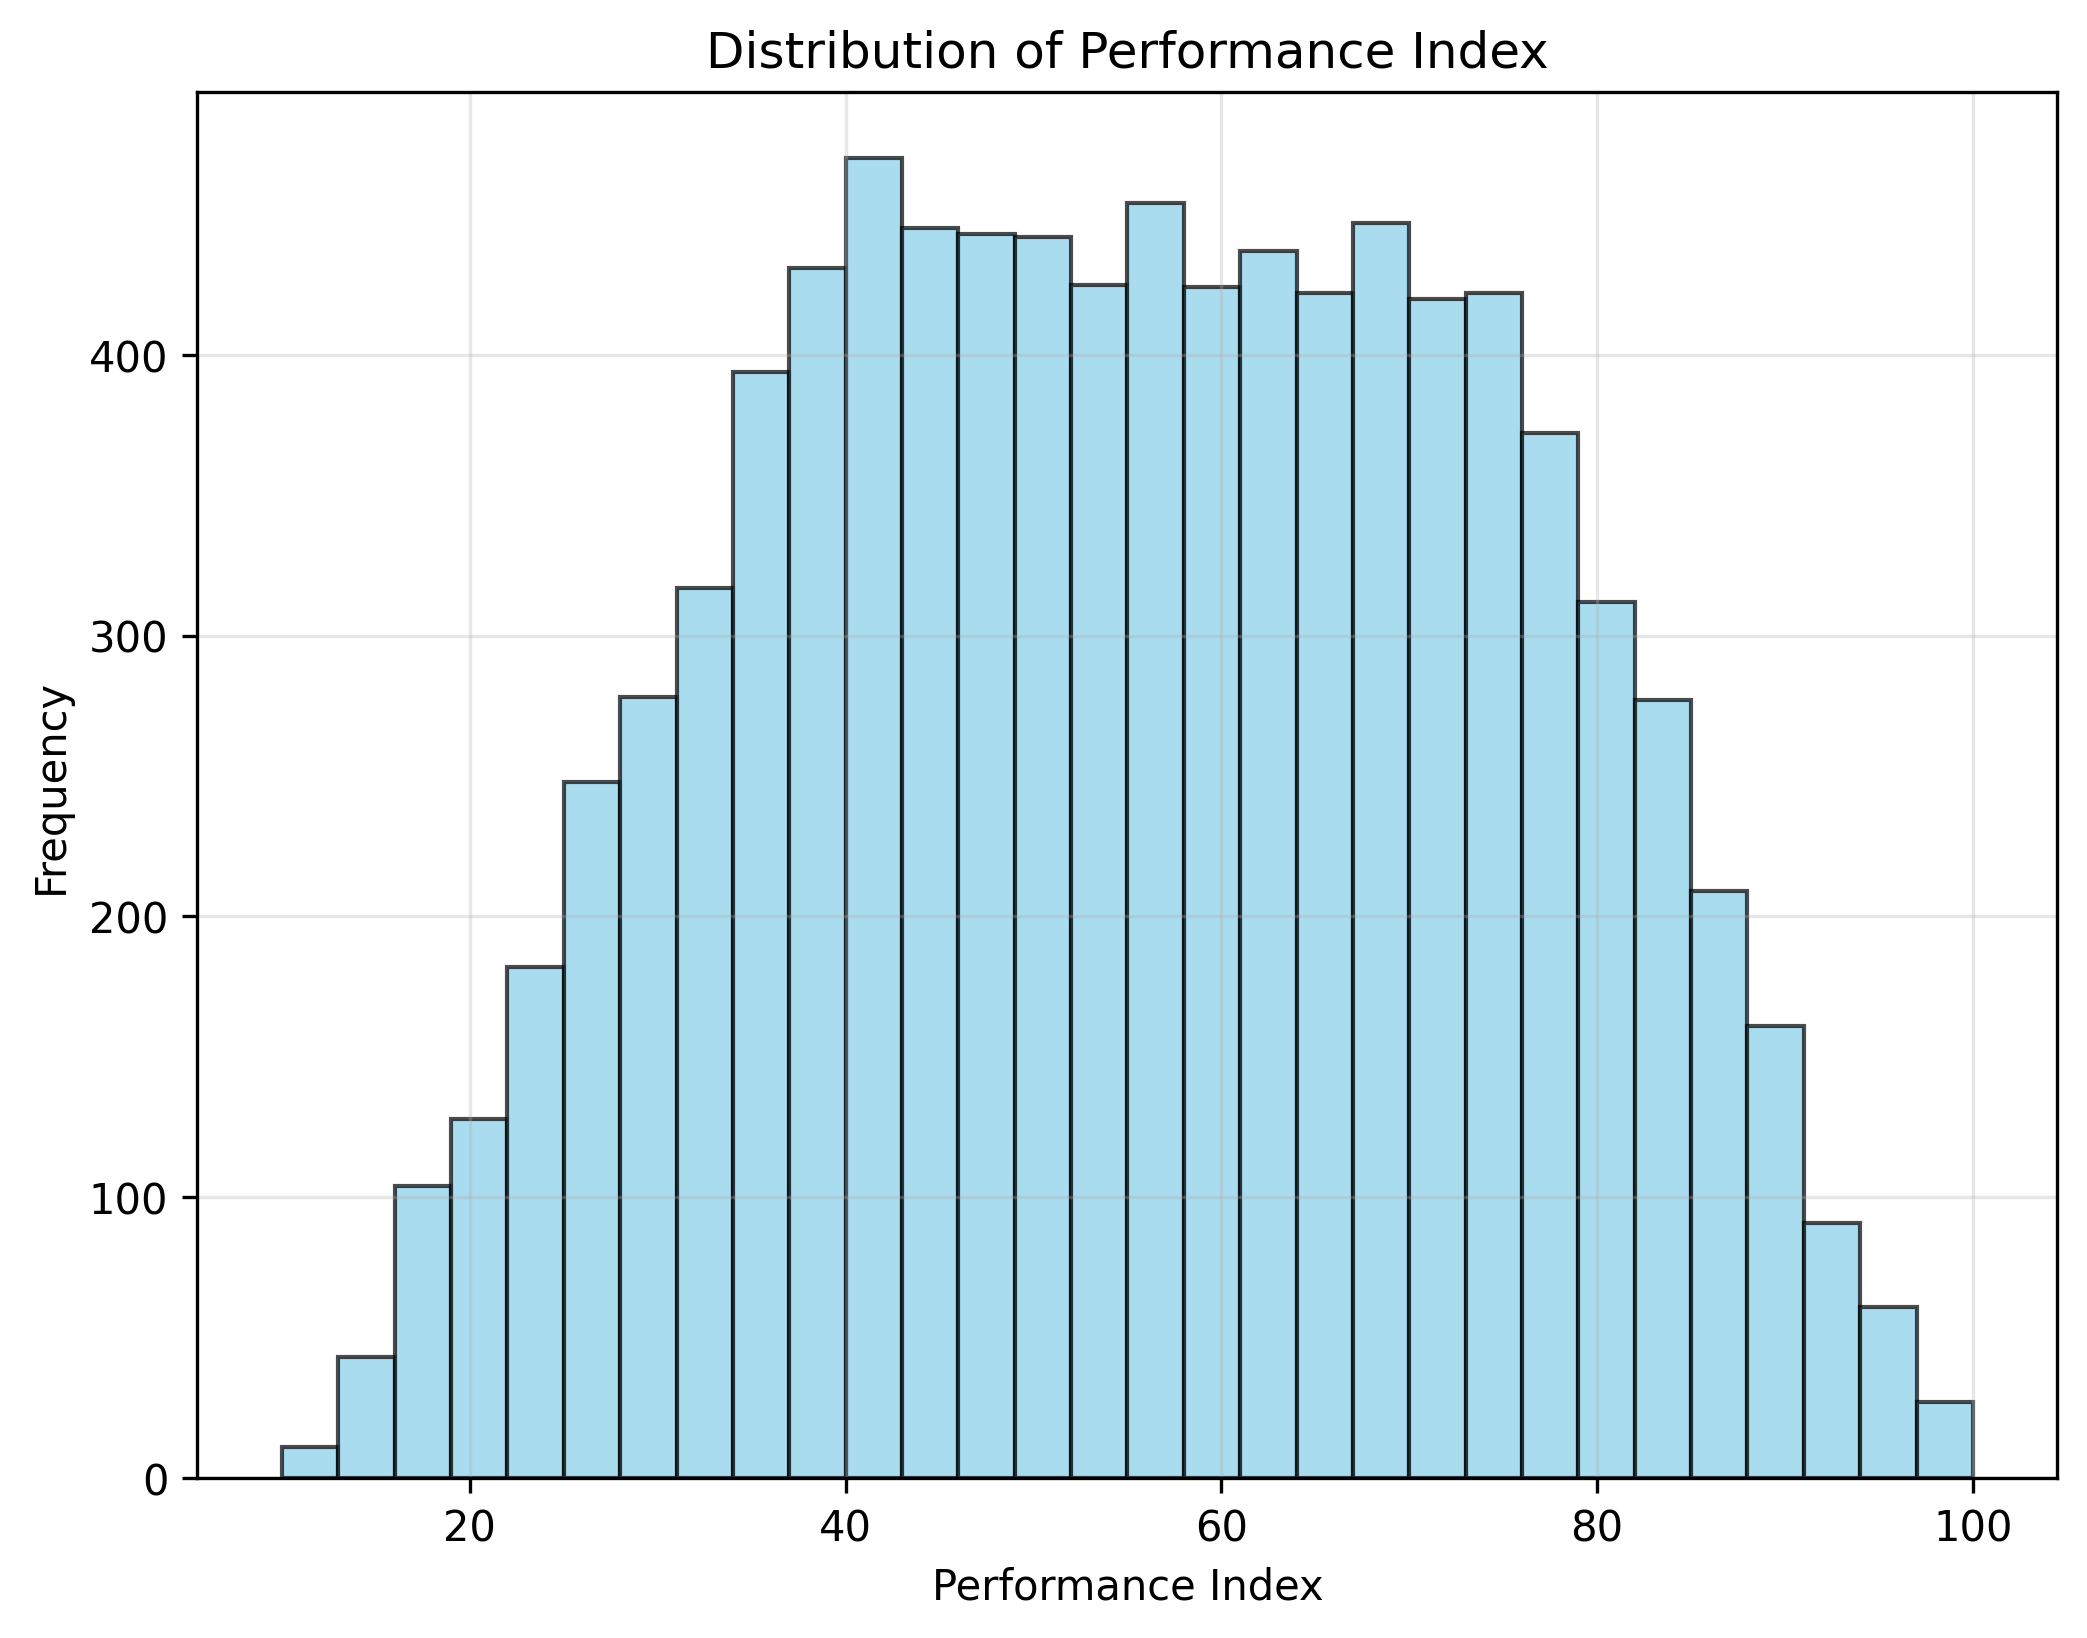
\includegraphics[width=0.7\textwidth]{imgs/figures/figure1_performance_index_distribution.png}
	\caption{Phân phối Performance Index}
	\label{fig:performance_distribution}
\end{figure}

\begin{itemize}
	\item \textbf{Nhận xét:}
	      \begin{itemize}
		      \item \textbf{Phân phối gần chuẩn}: Biểu đồ histogram cho thấy Performance Index có phân phối gần như chuẩn với đỉnh tại khoảng 40-45 điểm.
		      \item \textbf{Tính đối xứng}: Phân phối tương đối đối xứng với độ lệch nhẹ về phía phải.
		      \item \textbf{Phạm vi rộng}: Dữ liệu phân bố từ khoảng 10 đến gần 100 điểm, cho thấy sự đa dạng lớn trong hiệu suất học tập.
		      \item \textbf{Tập trung chính}: Phần lớn sinh viên có điểm số trong khoảng 30-70, với mật độ cao nhất ở khoảng 40-50 điểm.
	      \end{itemize}
\end{itemize}

\begin{figure}[H]
	\centering
	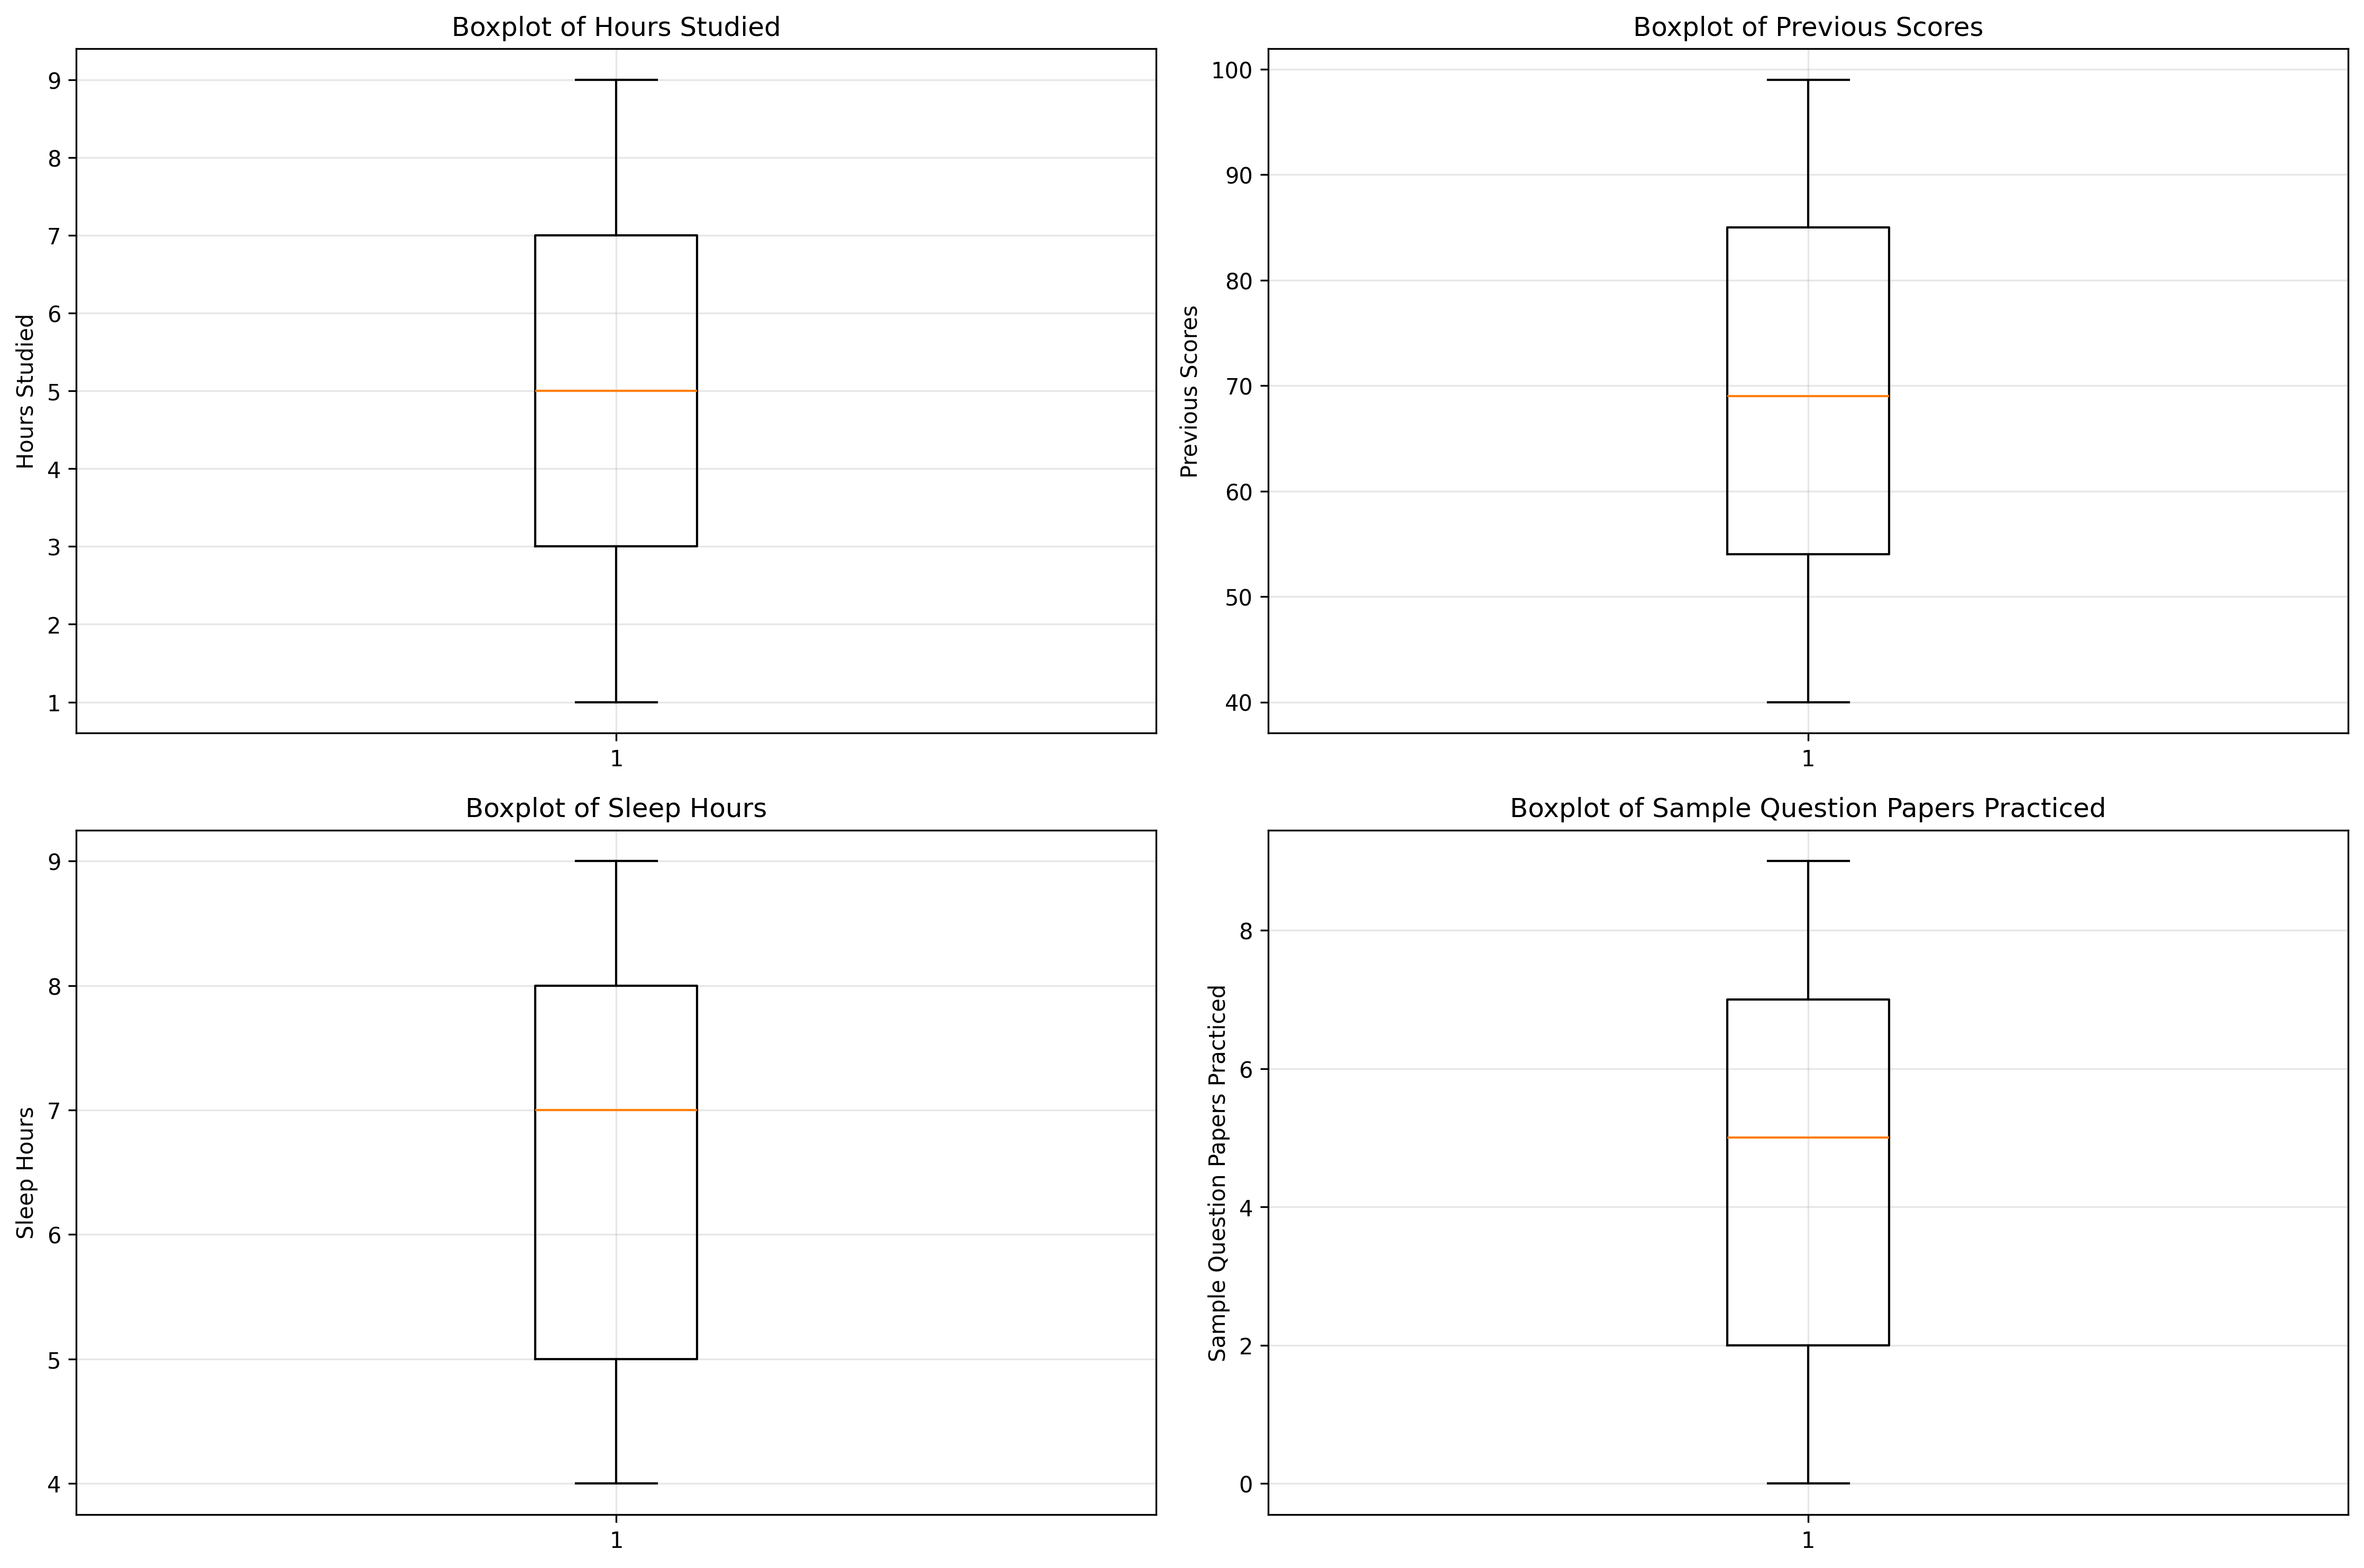
\includegraphics[width=0.9\textwidth]{imgs/figures/figure2_boxplots_numerical_features.png}
	\caption{Biểu đồ hộp các đặc trưng số}
	\label{fig:boxplots}
\end{figure}

\begin{itemize}
	\item \textbf{Nhận xét:}
	      \begin{itemize}
		      \item \textbf{Hours Studied}: Phân phối đối xứng với trung vị khoảng 5 giờ, IQR từ 3-7 giờ, phạm vi từ 1-9 giờ. Không có outliers đáng kể.
		      \item \textbf{Previous Scores}: Phân phối đối xứng với trung vị khoảng 70 điểm, IQR từ 55-85 điểm, phạm vi từ 40-100 điểm. Phân phối cân bằng và ổn định.
		      \item \textbf{Sleep Hours}: Phân phối đối xứng với trung vị khoảng 7 giờ, IQR từ 5-8 giờ, phạm vi từ 4-9 giờ. Phân bố khá tập trung.
		      \item \textbf{Sample Question Papers}: Phân phối đối xứng với trung vị khoảng 5 đề, IQR từ 2-7 đề, phạm vi từ 0-9 đề. Có một số sinh viên không luyện đề (giá trị 0).
	      \end{itemize}
\end{itemize}

\begin{figure}[H]
	\centering
	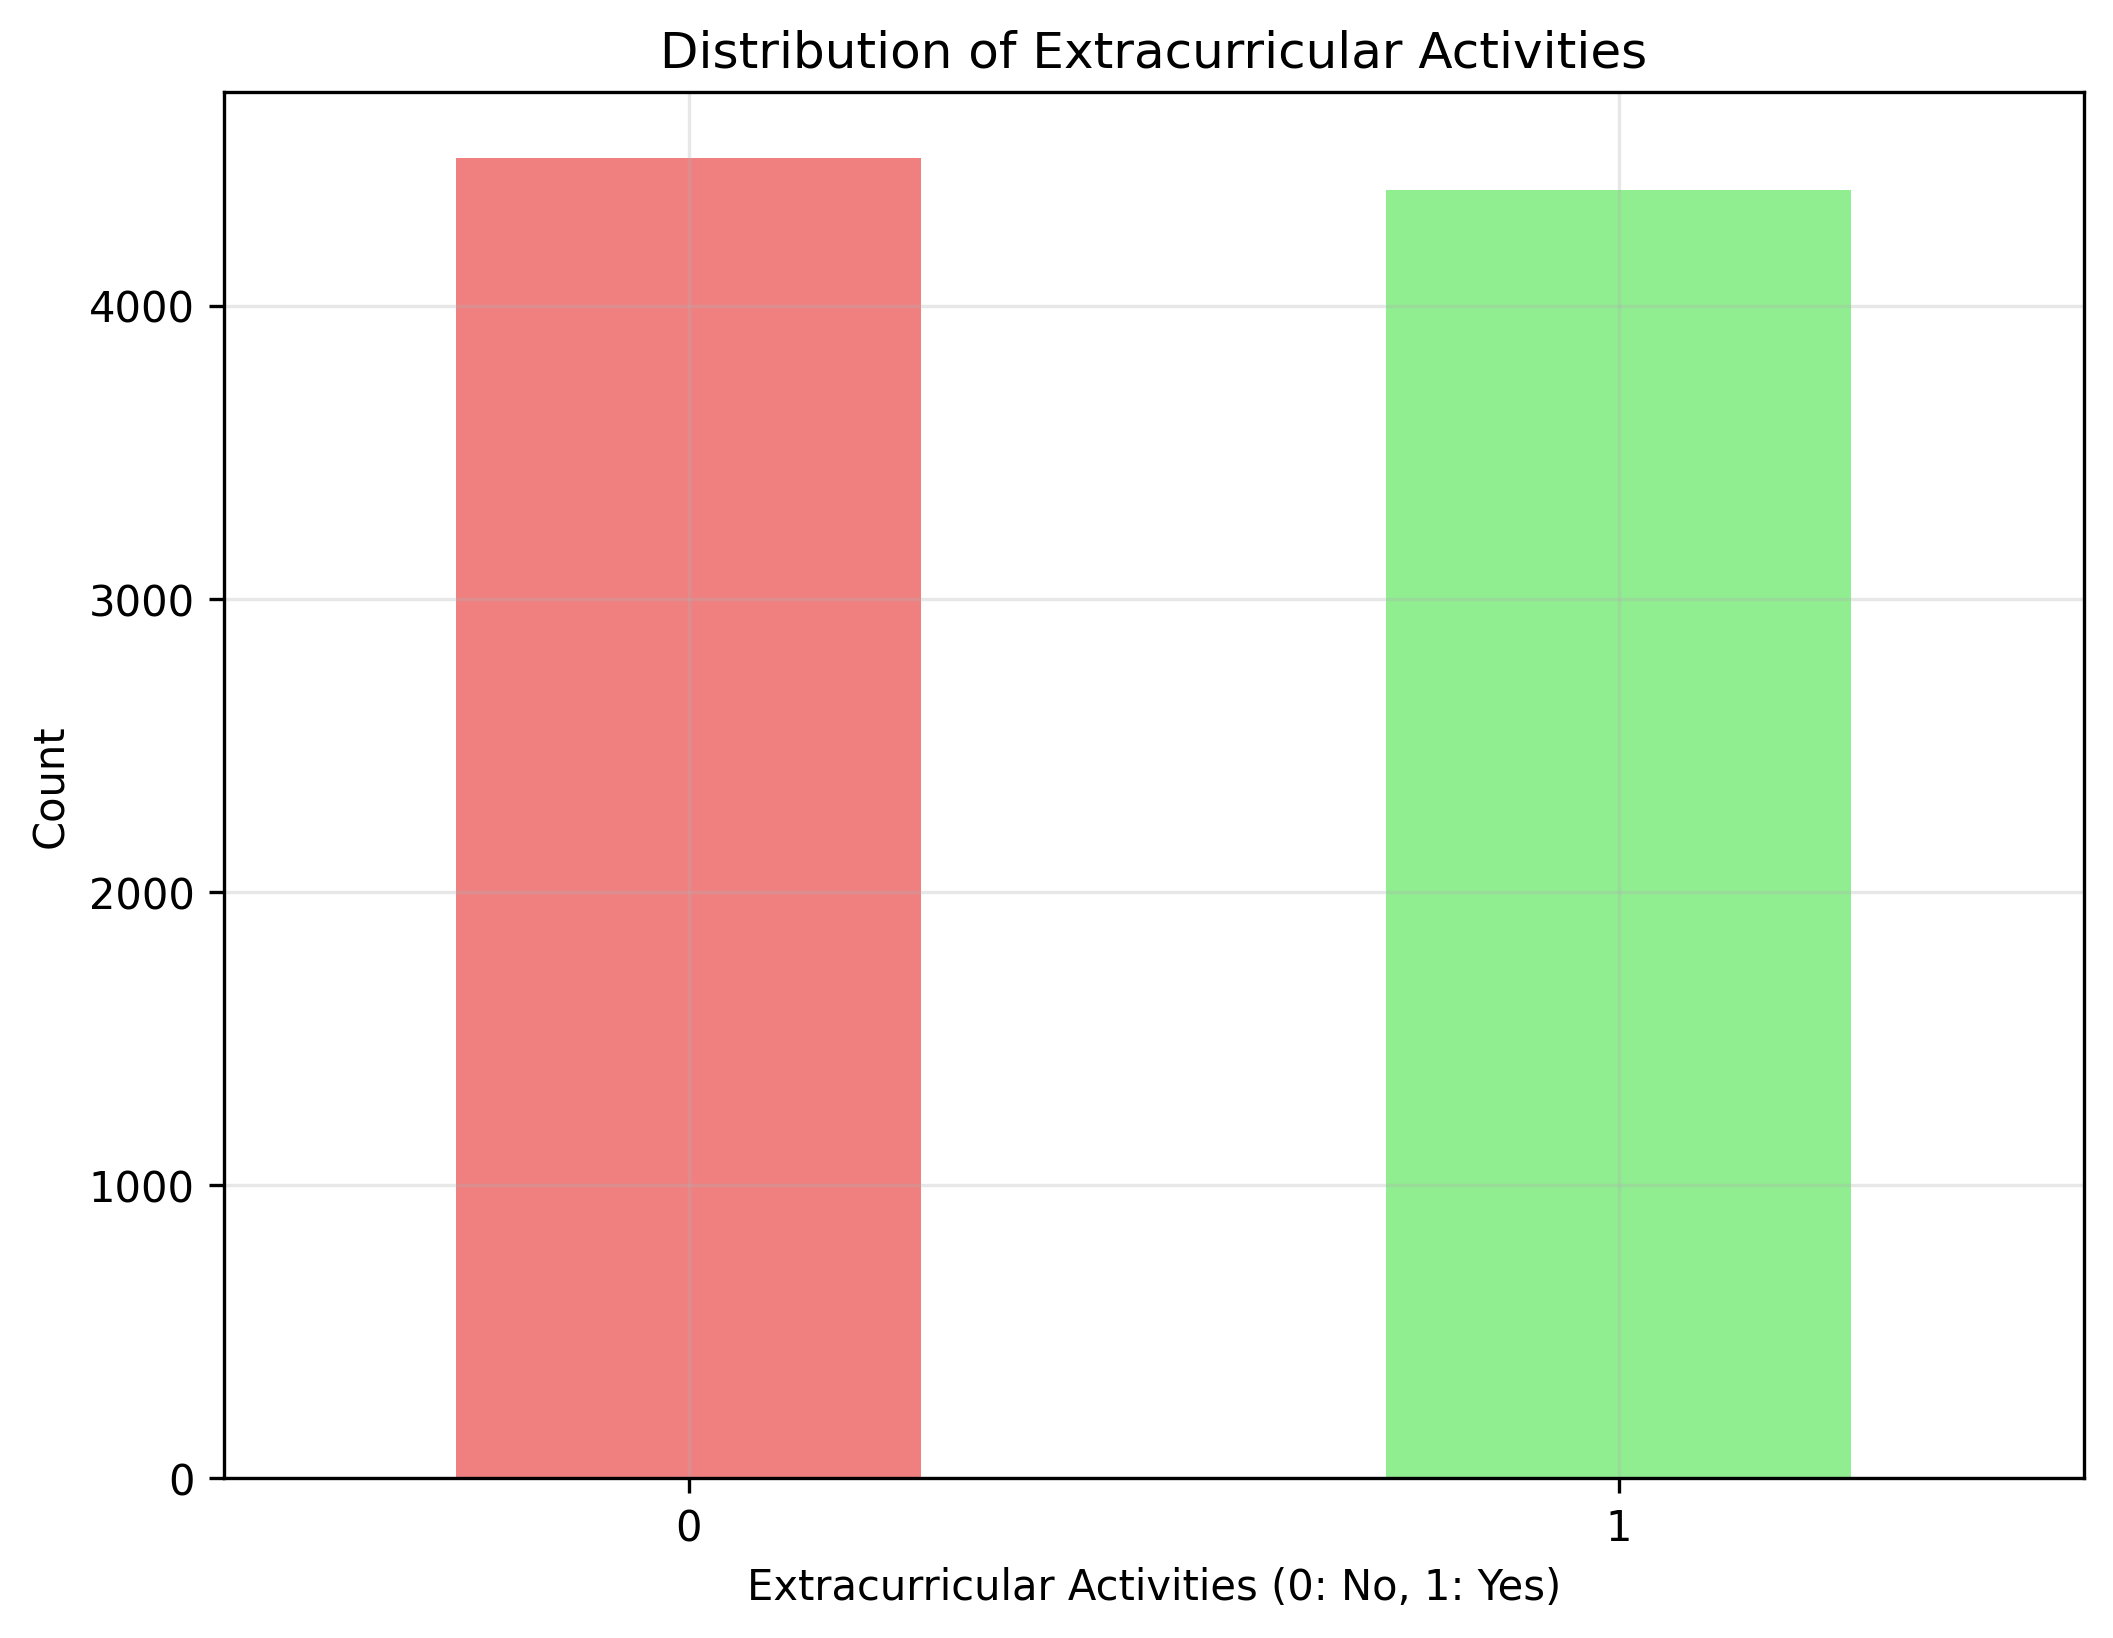
\includegraphics[width=0.7\textwidth]{imgs/figures/figure3_extracurricular_activities_distribution.png}
	\caption{Phân phối Hoạt động Ngoại khóa}
	\label{fig:extracurricular}
\end{figure}

\begin{itemize}
	\item \textbf{Nhận xét:}
	      \begin{itemize}
		      \item \textbf{Phân bố cân bằng}: Số lượng sinh viên tham gia và không tham gia hoạt động ngoại khóa gần như bằng nhau.
		      \item \textbf{Tính đại diện}: Sự cân bằng này đảm bảo dữ liệu có tính đại diện tốt, tránh thiên lệch trong phân tích.
	      \end{itemize}
\end{itemize}

\begin{figure}[H]
	\centering
	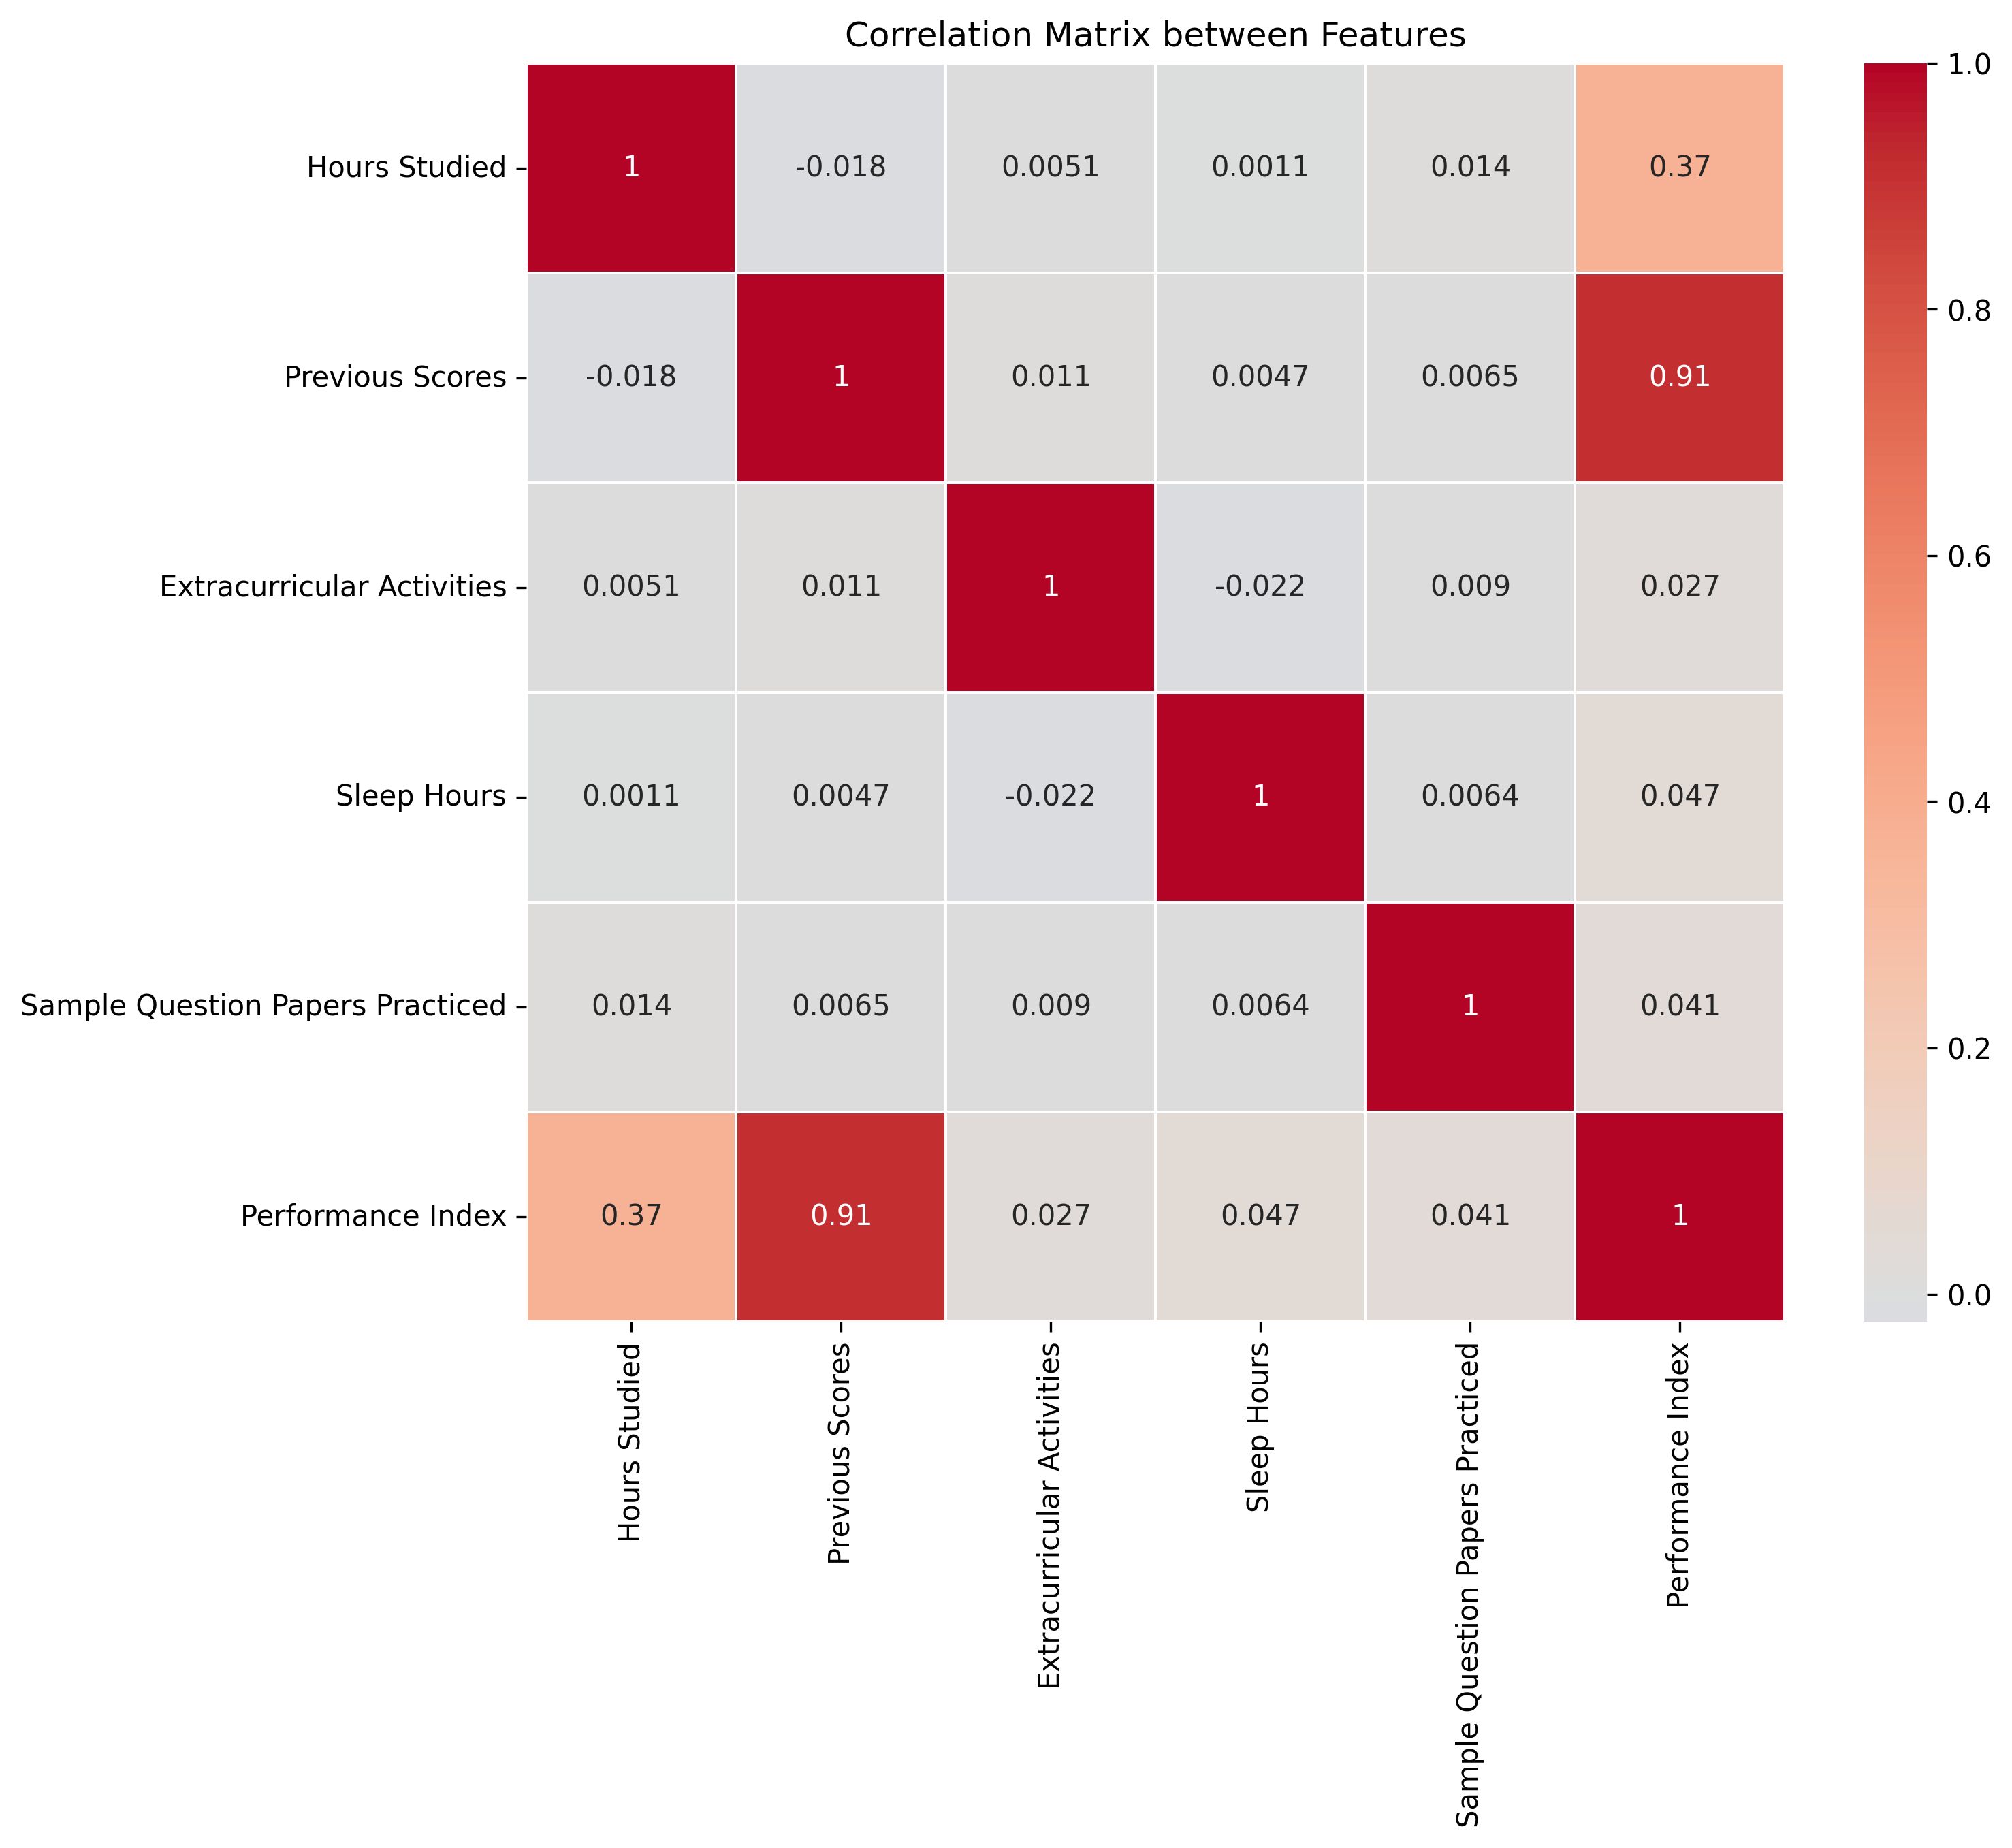
\includegraphics[width=0.9\textwidth]{imgs/figures/figure4_correlation_matrix.png}
	\caption{Ma trận tương quan giữa các đặc trưng}
	\label{fig:correlation}
\end{figure}

\begin{itemize}
	\item \textbf{Nhận xét:}
	      \begin{itemize}
		      \item Previous Scores có tương quan rất mạnh với Performance Index (0.91) → Điểm số trước đây dự đoán tốt hiệu suất.
		      \item Hours Studied có tương quan dương vừa phải với Performance Index (0.37) → Học nhiều giờ giúp cải thiện hiệu suất, nhưng không mạnh bằng điểm số trước.
		      \item Các biến khác (Extracurricular Activities, Sleep Hours, Sample Question Papers Practiced) hầu như không có tương quan đáng kể với Performance Index (< 0.05).
	      \end{itemize}
\end{itemize}

\begin{figure}[H]
	\centering
	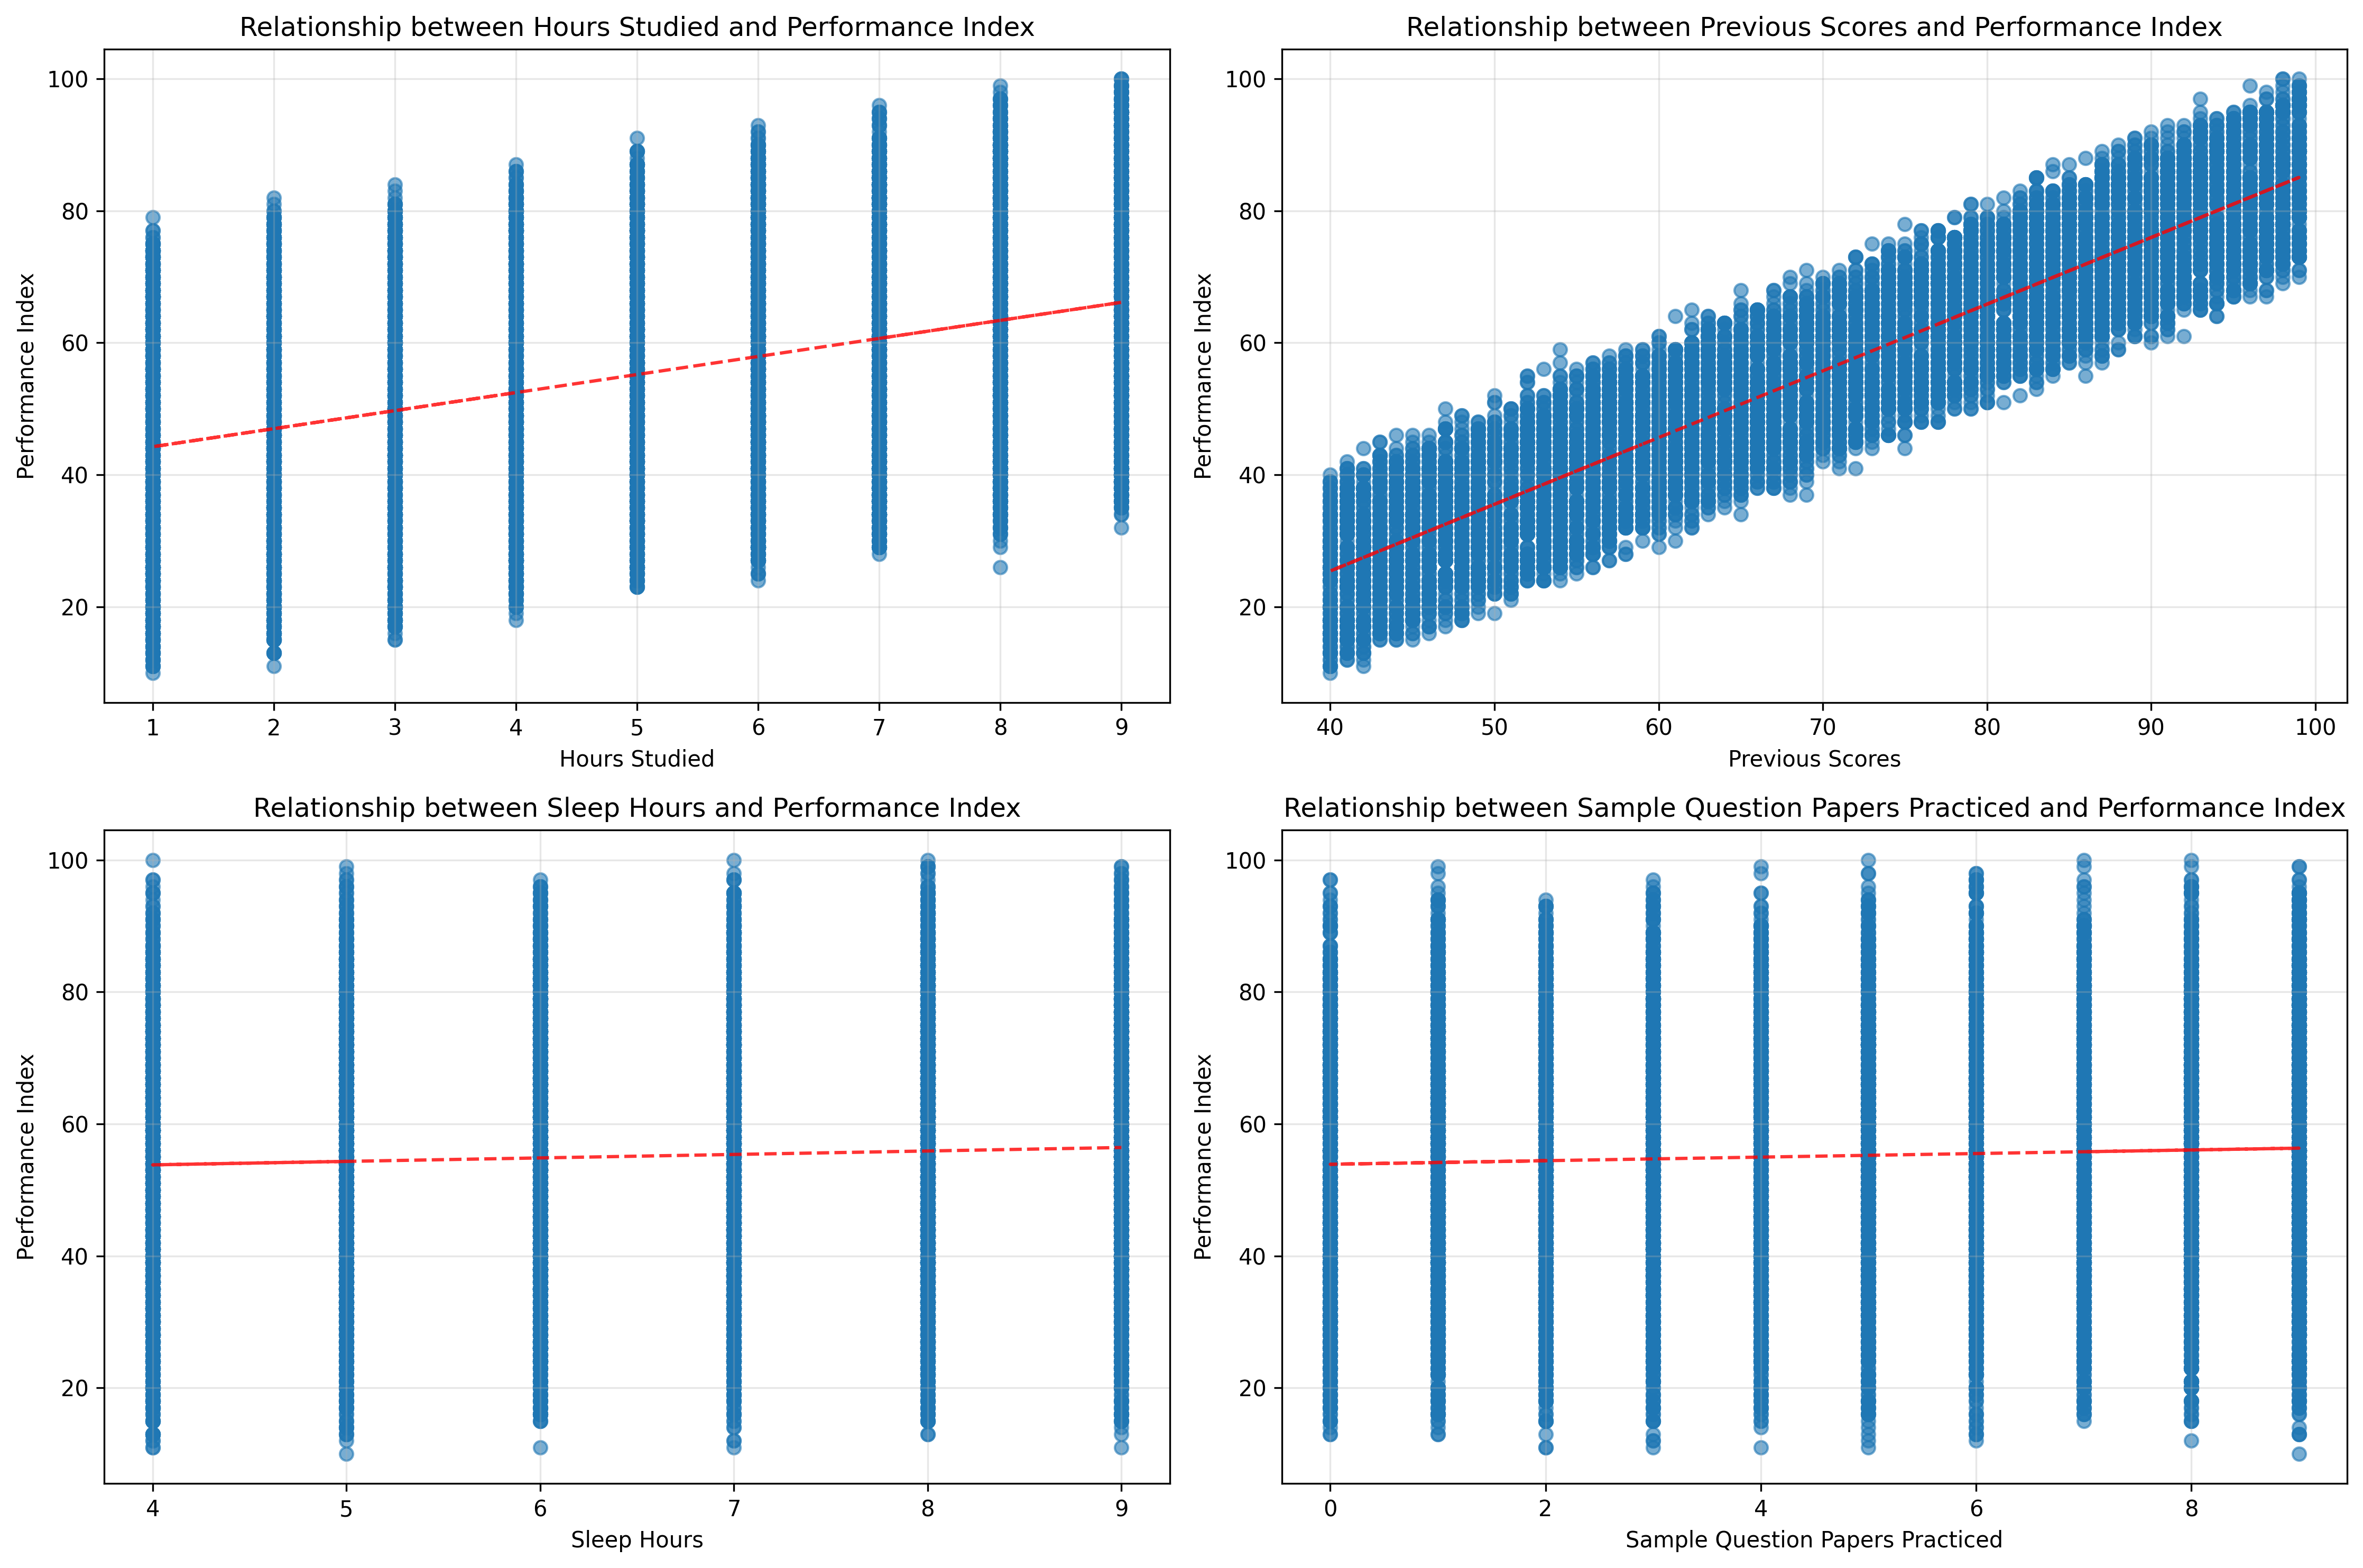
\includegraphics[width=0.9\textwidth]{imgs/figures/figure5_scatter_plots_relationships.png}
	\caption{Biểu đồ phân tán mối quan hệ với Performance Index}
	\label{fig:scatter}
\end{figure}

\begin{itemize}
	\item \textbf{Nhận xét:}
	      \begin{itemize}
		      \item \textbf{Previous Scores}: Có mối quan hệ tuyến tính mạnh và rõ ràng với Performance Index. Đường hồi quy cho thấy correlation coefficient cao, với sự phân bố dữ liệu khá sát đường thẳng.
		      \item \textbf{Hours Studied}: Mối quan hệ tuyến tính yếu hơn nhưng vẫn rõ ràng. Có xu hướng tăng nhẹ theo thời gian học, nhưng độ phân tán lớn hơn Previous Scores.
		      \item \textbf{Sleep Hours}: Mối quan hệ rất yếu hoặc không có correlation rõ ràng. Đường hồi quy gần như nằm ngang, cho thấy Sleep Hours ít ảnh hưởng đến Performance Index.
		      \item \textbf{Sample Question Papers Practiced}: Tương tự Sleep Hours, mối quan hệ rất yếu với đường hồi quy gần như nằm ngang, cho thấy việc luyện tập đề mẫu không có tác động mạnh đến hiệu suất tổng thể.
	      \end{itemize}
\end{itemize}

\begin{figure}[H]
	\centering
	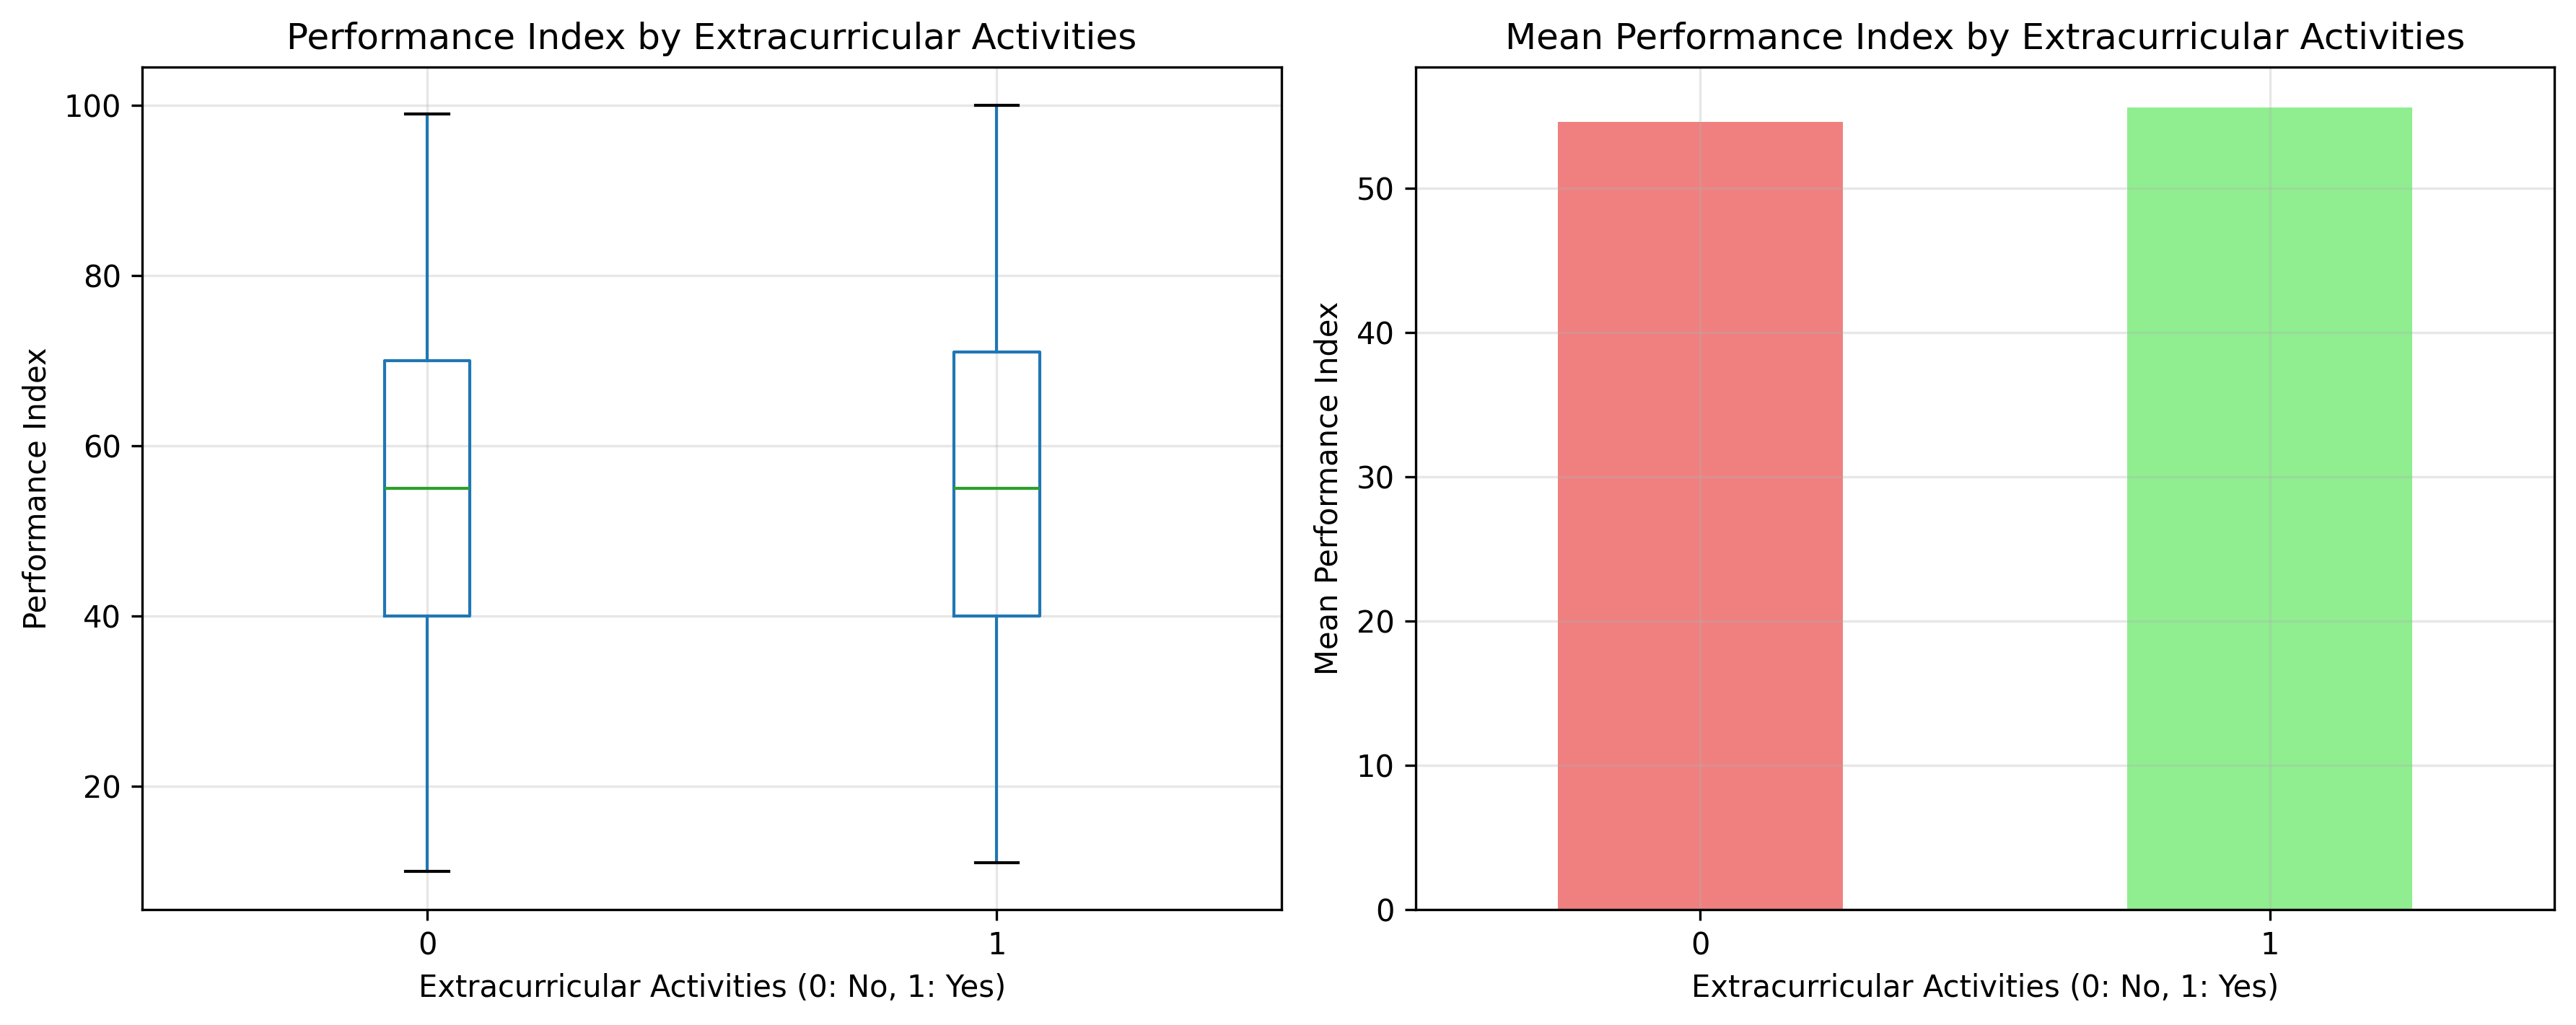
\includegraphics[width=0.9\textwidth]{imgs/figures/figure6_performance_by_extracurricular.png}
	\caption{So sánh hiệu suất theo hoạt động ngoại khóa}
	\label{fig:performance_comparison}
\end{figure}

\begin{itemize}
	\item \textbf{Nhận xét:}
	      \begin{itemize}
		      \item \textbf{Phân phối tương tự nhau}: Từ biểu đồ boxplot, cả hai nhóm (có và không có hoạt động ngoại khóa) đều có phân phối Performance Index khá tương đồng với median gần như bằng nhau (khoảng 55 điểm).
		      \item \textbf{Độ biến thiên tương đương}: Khoảng tứ phân vị (IQR) của cả hai nhóm gần như bằng nhau, cho thấy độ phân tán dữ liệu tương tự.
		      \item \textbf{Chênh lệch mean nhẹ}: Biểu đồ cột cho thấy sinh viên tham gia hoạt động ngoại khóa (nhóm 1) có điểm trung bình cao hơn một chút so với nhóm không tham gia (nhóm 0), nhưng sự khác biệt không lớn (khoảng 1-2 điểm).
		      \item \textbf{Tác động hạn chế}: Mặc dù có sự khác biệt về mean, nhưng sự chồng lấn lớn giữa hai phân phối cho thấy hoạt động ngoại khóa có tác động tích cực nhưng không quá mạnh đến hiệu suất học tập.
	      \end{itemize}
\end{itemize}

\subsection{Kết quả các Mô hình Hồi quy Tuyến tính}

\subsubsection{Yêu cầu 2a: Mô hình 5 đặc trưng}

\textbf{Công thức mô hình}:
\begin{align}
	\text{Performance} & = -33.961 + 2.852 \times \text{Hours Studied} \nonumber          \\
	                   & \quad + 1.018 \times \text{Previous Scores} \nonumber            \\
	                   & \quad + 0.606 \times \text{Extracurricular Activities} \nonumber \\
	                   & \quad + 0.473 \times \text{Sleep Hours} \nonumber                \\
	                   & \quad + 0.192 \times \text{Sample Question Papers}
\end{align}

\textbf{Kết quả đánh giá}:
\begin{itemize}
	\item \textbf{MSE trên tập kiểm tra}: 4.092356
	\item \textbf{Nhận xét}: Mô hình sử dụng toàn bộ 5 đặc trưng cho kết quả khá tốt, với Previous Scores và Hours Studied có trọng số cao nhất.
\end{itemize}

\subsubsection{Yêu cầu 2b: Mô hình đặc trưng tốt nhất}

\textbf{Kết quả k-fold Cross Validation}:

\begin{table}[H]
	\centering
	\begin{tabular}{|c|l|c|}
		\hline
		\textbf{STT} & \textbf{Mô hình với 1 đặc trưng} & \textbf{MSE} \\
		\hline
		1            & Hours Studied                    & 317.510929   \\
		\hline
		2            & Previous Scores                  & 60.141086    \\
		\hline
		3            & Extracurricular Activities       & 367.670027   \\
		\hline
		4            & Sleep Hours                      & 367.287602   \\
		\hline
		5            & Sample Question Papers Practiced & 367.485440   \\
		\hline
	\end{tabular}
	\caption{Kết quả Cross Validation cho mô hình 1 đặc trưng}
	\label{tab:single_feature}
\end{table}

\textbf{Đặc trưng tốt nhất}: Previous Scores với MSE = 60.141086

\textbf{Công thức mô hình}:
\begin{equation}
	\text{Performance} = -15.015 + 1.011 \times \text{Previous Scores}
\end{equation}

\textbf{Kết quả đánh giá}:
\begin{itemize}
	\item \textbf{MSE trên tập kiểm tra}: 58.906757
	\item \textbf{Giải thích}: Previous Scores là đặc trưng quan trọng nhất vì nó phản ánh trực tiếp năng lực học tập trước đó của sinh viên, có tương quan mạnh với kết quả hiện tại.
\end{itemize}

\subsubsection{Yêu cầu 2c: Mô hình tùy chỉnh}

\textbf{Các mô hình được thiết kế}:

\begin{table}[H]
	\centering
	\begin{tabular}{|c|l|c|}
		\hline
		\textbf{STT} & \textbf{Mô hình}                & \textbf{MSE} \\
		\hline
		1            & 2 đặc trưng tốt nhất            & 5.220514     \\
		\hline
		2            & 3 đặc trưng tốt nhất            & 5.136711     \\
		\hline
		3            & Đặc trưng đa thức               & 60.180196    \\
		\hline
		4            & Đặc trưng chuẩn hóa z-score     & 5.220514     \\
		\hline
		5            & Đặc trưng tương tác và kỹ thuật & 18.505961    \\
		\hline
	\end{tabular}
	\caption{Kết quả Cross Validation cho các mô hình tùy chỉnh}
	\label{tab:custom_models}
\end{table}

\textbf{Mô hình tốt nhất}: Model 2 (Top 3 features) với MSE = 5.136711

\textbf{Công thức mô hình}:
\begin{align}
	\text{Performance} & = -30.019 + 2.855 \times \text{Hours Studied} \nonumber \\
	                   & \quad + 1.018 \times \text{Previous Scores} \nonumber   \\
	                   & \quad + 0.580 \times \text{Extracurricular Activities}
\end{align}

\textbf{Kết quả đánh giá}:
\begin{itemize}
	\item \textbf{MSE trên tập kiểm tra}: 5.273269
	\item \textbf{Giải thích}: Mô hình kết hợp 3 đặc trưng quan trọng nhất cho kết quả tốt nhất, loại bỏ được nhiễu từ các đặc trưng ít quan trọng.
\end{itemize}

\subsection{Phân tích và So sánh các Mô hình}

\subsubsection{Bảng tổng hợp kết quả}

\begin{table}[H]
	\centering
	\begin{tabular}{|l|c|c|}
		\hline
		\textbf{Mô hình}                & \textbf{MSE Cross Validation} & \textbf{MSE Test} \\
		\hline
		Mô hình 5 đặc trưng (2a)        & -                             & 4.092356          \\
		\hline
		Đặc trưng tốt nhất (2b)         & 60.141086                     & 58.906757         \\
		\hline
		Mô hình tùy chỉnh tốt nhất (2c) & 5.136711                      & 5.273269          \\
		\hline
	\end{tabular}
	\caption{So sánh kết quả các mô hình}
	\label{tab:model_comparison}
\end{table}

\subsubsection{Nhận xét về hiệu suất}

\textbf{Thứ tự hiệu suất (từ tốt đến kém)}:
\begin{enumerate}
	\item \textbf{Mô hình 5 đặc trưng (2a)}: MSE = 4.092356
	\item \textbf{Mô hình tùy chỉnh tốt nhất (2c)}: MSE = 5.273269
	\item \textbf{Đặc trưng tốt nhất (2b)}: MSE = 58.906757
\end{enumerate}

\textbf{Phân tích hiệu suất}:
\begin{itemize}
	\item Mô hình 5 đặc trưng (2a) đạt hiệu suất tốt nhất với MSE thấp nhất, cho thấy sự đóng góp tích cực của tất cả các đặc trưng
	\item Mô hình tùy chỉnh (2c) có hiệu suất tốt thứ hai, chứng tỏ việc lựa chọn đặc trưng thông minh có thể cạnh tranh với mô hình đầy đủ
	\item Mô hình 1 đặc trưng (2b) có hiệu suất thấp nhất do hạn chế thông tin đầu vào
\end{itemize}

\subsection{Kết luận cuối cùng}
Những yếu tố quan trọng ảnh hưởng đến thành tích học tập theo thứ tự ưu tiên:
\begin{enumerate}
	\item \textbf{Previous Scores}: Yếu tố quan trọng nhất, phản ánh nền tảng kiến thức
	\item \textbf{Hours Studied}: Thời gian học tập có tác động mạnh đến kết quả
	\item \textbf{Extracurricular Activities}: Hoạt động ngoại khóa góp phần nâng cao hiệu suất học tập
	\item \textbf{Sleep Hours}: Có tác động nhưng không mạnh bằng các yếu tố trên
	\item \textbf{Sample Question Papers Practiced}: Tác động thấp nhất trong các yếu tố được khảo sát
\end{enumerate}




\newpage
\section{Acknowledgement}

Đồ án có sự hỗ trợ của \textbf{GitHub Copilot} trong việc:
\begin{itemize}
	\item Viết docstrings cho các hàm Python
	\item Tối ưu hóa code và xử lý lỗi
	\item Tạo comments giải thích cho các đoạn code phức tạp
	\item Hỗ trợ viết báo cáo LaTeX với định dạng chuẩn
	\item So sánh các mô hình 
\end{itemize}

\textbf{Lưu ý}: Tất cả logic chính, thuật toán Linear Regression, k-fold Cross Validation và Feature Engineering đều được tự thiết kế và cài đặt. AI chỉ hỗ trợ về mặt cú pháp và định dạng.


\begin{thebibliography}{9}

  \bibitem{boyd_vandenberghe}
  Boyd, S. \& Vandenberghe, L.,
  \textit{Introduction to Applied Linear Algebra -- Vectors, Matrices, and Least Squares}, Chương 13: Least squares, Cambridge University Press, 2018.
  \newline
  \url{https://web.stanford.edu/~boyd/vmls/vmls.pdf}

  \bibitem{cross_validation}
  Scikit-learn developers,
  \textit{Cross-validation: evaluating estimator performance}, scikit-learn Documentation.
  \newline
  \url{https://scikit-learn.org/stable/modules/cross_validation.html}

  \bibitem{normal_equation}
  Andrew Ng,
  \textit{Machine Learning Course - Normal Equation}, Stanford CS229 Lecture Notes.
  \newline
  \url{https://cs229.stanford.edu/notes2020fall/notes2020fall/cs229-notes1.pdf}

  \bibitem{mse_evaluation}
  Wikipedia,
  \textit{Mean squared error}, truy cập ngày 13/08/2025.
  \newline
  \url{https://en.wikipedia.org/wiki/Mean_squared_error}

\end{thebibliography}



\pagebreak
\end{document}